\chapter{Aromaticiteit en elektrofiele aromatische substitutie}\label{ch:b2:aromatic-substitution}

Broomwater verliest binnen enkele seconden zijn kleur als je het met een alkeen schudt,
en helemaal niet met benzeen. Toch reageert benzeen wel met broom zodra er een
beetje ijzer(III)bromide bij komt --- en het product, broombenzeen, heeft nog steeds
zijn \omterm{def:b2:huckel:aromatic}{aromatische} zesring: één waterstofatoom is vervangen, er is niets
geaddeerd. \omterm{def:b2:huckel:aromatic}{Aromatische} ringen substitueren in plaats van te adderen, omdat additie
de stabilisatie zou weggooien die in \cref{ch:b2:huckel} berekend werd. Hetzelfde
mechanisme nitreert, sulfoneert, alkyleert en acyleert benzeenringen, en
de groepen die al op een ring zitten bepalen, met verrassende regelmaat, waar de
volgende terechtkomt.

\begin{recall}
\Cref{ch:b2:huckel}: aromaticiteit en de \omterm{def:b2:huckel:delocalisation}{delokalisatie-energie} van benzeen. Het deel van jaar~1:
elektrofiele addities aan alkenen, inductieve en mesomere effecten, donor- en
acceptorgroepen, carbokationen en hun omleggingen, het postulaat van Hammond, lewiszuren,
energieprofielen.
\end{recall}

\begin{omfigure}
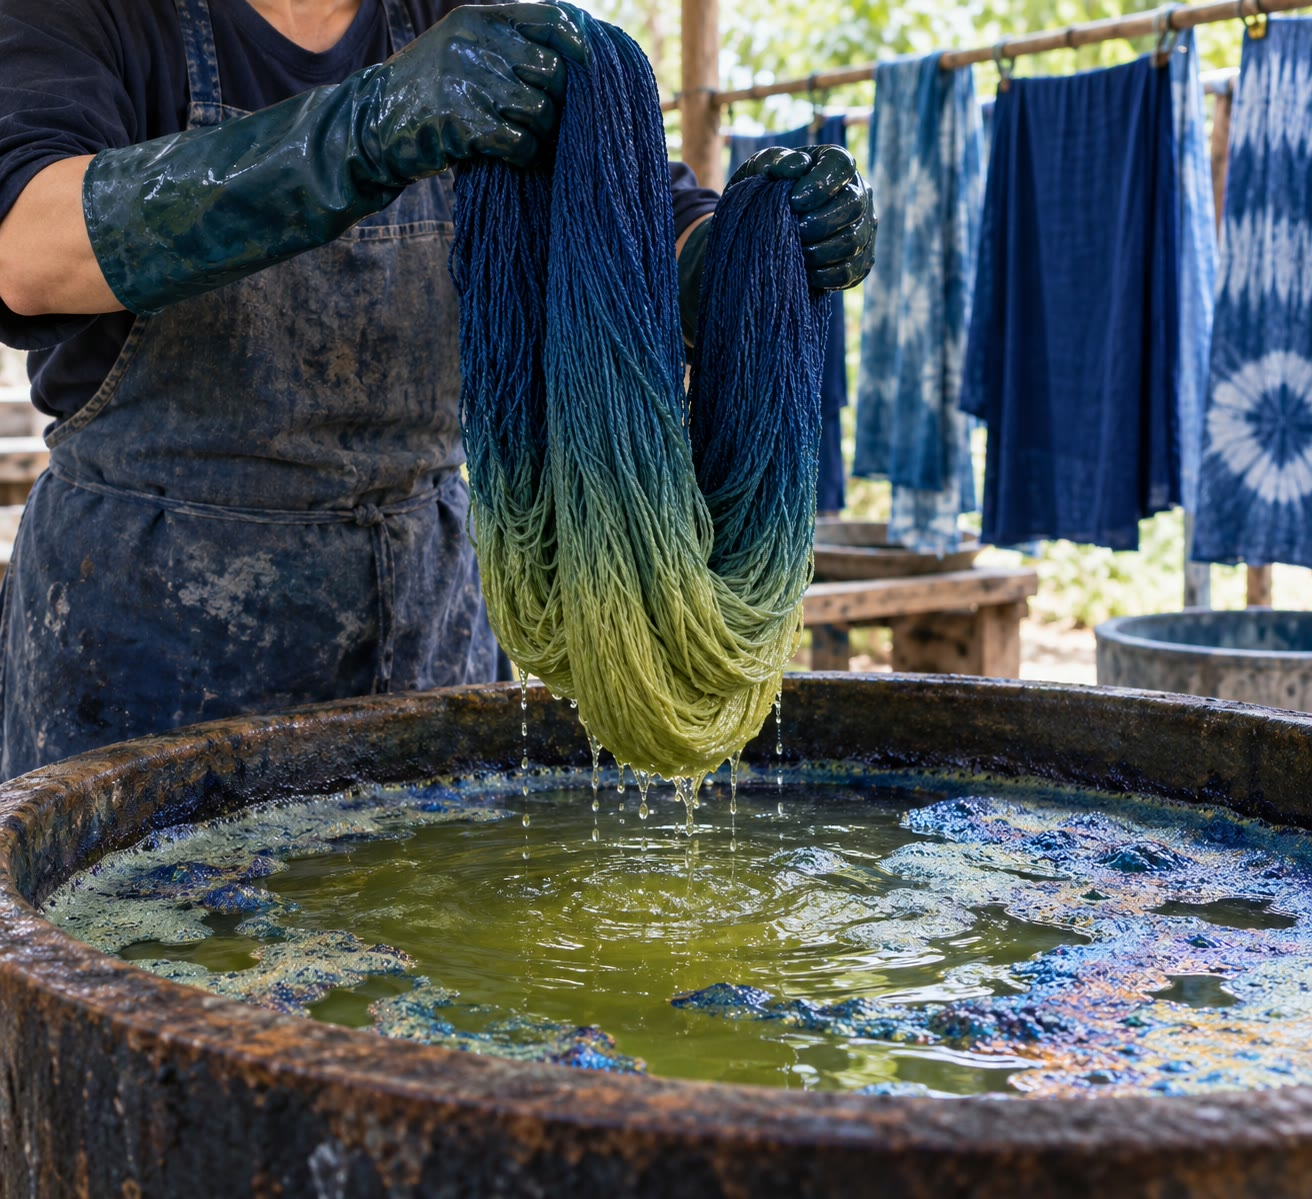
\includegraphics[width=0.55\linewidth]{images/book3/ai/b2-22-indigo-vat-2.jpg}

{\small Garen verven in een indigokuip (illustratie). Het garen komt geelgroen uit de kuip, doordrenkt
met de oplosbare gereduceerde vorm van de kleurstof, en wordt blauw aan de lucht doordat zuurstof het terug omzet in
onoplosbaar indigo. Indigo is, zoals de meeste kleurstoffen, opgebouwd uit \omterm{def:b2:huckel:aromatic}{aromatische} ringen;
de kleurstofindustrie van de negentiende eeuw groeide uit de substitutiereacties van dit
hoofdstuk, toegepast op benzeen uit steenkoolteer.}
\end{omfigure}

\section{Substitutie, geen additie}

\begin{definition}[Areen]\label{def:b2:aromatic-substitution:arene}
Een \emph{areen}\index{areen} is een koolwaterstof met ten minste één \omterm{def:b2:huckel:aromatic}{aromatische} ring, zoals
benzeen, tolueen (methylbenzeen) of naftaleen; een arylgroep (\ce{Ar}) is een areen min
één waterstofatoom.
\end{definition}

\begin{proposition}[Waarom benzeen niet addeert]\label{prop:b2:aromatic-substitution:no-addition}
Een additie aan benzeen zou de \omterm{def:b2:huckel:aromatic}{aromatische} ring omzetten in een \omterm{def:b2:huckel:aromatic}{niet-aromatisch} cyclohexadieen en
het grootste deel van de \qty{150}{kJ/mol} \omterm{def:b2:huckel:aromatic}{aromatische} stabilisatie verliezen; substitutie behoudt die.
\end{proposition}

\begin{proof}[Redenering]
In \cref{ch:b2:huckel} bleek de hydrogenering van benzeen tot cyclohexa-1,3-dieen
\omterm{def:b2:reaction-enthalpy:exothermic}{endotherm} (\qty{+22}{kJ/mol}, uit \qty{-206.0}{} en \qty{-227.7}{kJ/mol}), terwijl die van een
gewone dubbele binding \qty{119}{kJ/mol} vrijmaakt: de eerste additie is de dure stap.
Na de eerste elektrofiele stap kan het gevormde kation ofwel een nucleofiel adderen, wat
een \omterm{def:b2:huckel:aromatic}{niet-aromatisch} \omterm{def:b2:frontier-orbitals:diels-alder}{dieen} achterlaat, ofwel een proton verliezen, wat de \omterm{def:b2:huckel:aromatic}{aromatische} ring herstelt. De tweede
weg is veel gunstiger.
% ledger: dfh:C6H6_g, dfh:C6H8_g, dfh:C6H10_g, dfh:C6H12_g
\end{proof}

\section{Het mechanisme}

\begin{definition}[Elektrofiele aromatische substitutie]\label{def:b2:aromatic-substitution:seAr}
Een \emph{elektrofiele aromatische substitutie}\index{elektrofiele aromatische substitutie}
vervangt een waterstofatoom van een \omterm{def:b2:huckel:aromatic}{aromatische} ring door een elektrofiel \ce{E+}. Het elektrofiel
bindt eerst aan één ringkoolstofatoom, wat een kation geeft waarin dat koolstofatoom tetraëdrisch is en de
positieve lading over de andere vijf verdeeld is: het \emph{whelandintermediair}\index{whelandintermediair}
(een areniumion). Een base haalt daarna het proton van het tetraëdrische koolstofatoom weg.
\end{definition}

\begin{proposition}[Twee stappen]\label{prop:b2:aromatic-substitution:mechanism}
De eerste stap, die de aromaticiteit vernietigt, is de trage; het verlies van het proton,
dat haar herstelt, is snel.
\end{proposition}

\begin{proof}[Redenering]
Het \omterm{def:b2:aromatic-substitution:seAr}{whelandintermediair} is een carbokation dat door delokalisatie over drie koolstofatomen gestabiliseerd is,
maar niet \omterm{def:b2:huckel:aromatic}{aromatisch}: het ligt hoog boven de reagentia, en volgens het postulaat van Hammond ligt de
overgangstoestand die ernaartoe leidt er qua structuur en energie dicht bij. De tweede stap
leidt omlaag naar een \omterm{def:b2:huckel:aromatic}{aromatisch} product: zijn barrière is laag.
\end{proof}

\begin{omfigure}
\begin{tikzpicture}
\begin{axis}[width=0.55\linewidth, height=5.4cm, xmin=-0.2, xmax=4.2, ymin=-5.5, ymax=11.5,
  axis x line=bottom, axis y line=left, xtick=\empty, ytick=\empty,
  xlabel={reactiecoördinaat}, ylabel={energie}, label style={font=\small}, clip=false]
\addplot[omDef, thick] table[x=x, y=sub] {figdata/out/bachelor-2-aromatic-profile.dat};
\addplot[omThm, thick, dashed, restrict x to domain=2:4] table[x=x, y=add] {figdata/out/bachelor-2-aromatic-profile.dat};
\node[font=\scriptsize, anchor=north west] at (axis cs:0.0,-0.6) {\ce{ArH + E+}};
\node[font=\scriptsize, anchor=north] at (axis cs:2,5.7) {Wheland};
\node[font=\scriptsize, anchor=west, omDef] at (axis cs:4.05,-4.0) {\ce{ArE + H+}};
\node[font=\scriptsize, anchor=west, omThm] at (axis cs:4.05,2.0) {additieproduct};
\node[font=\scriptsize, anchor=south] at (axis cs:1,10.1) {traag};
\end{axis}
\end{tikzpicture}

{\small Energieprofiel van een \omterm{def:b2:aromatic-substitution:seAr}{elektrofiele aromatische substitutie}, schematisch (een model).
De eerste stap, die het \omterm{def:b2:aromatic-substitution:seAr}{whelandintermediair} vormt, heeft de hoogste barrière. Verlies van een
proton (doorgetrokken) herstelt de \omterm{def:b2:huckel:aromatic}{aromatische} ring; additie van een nucleofiel (gestreept) zou een
product boven de reagentia achterlaten.}
\end{omfigure}

\begin{omfigure}
\setchemfig{atom sep=2em}
\schemestart
\chemfig{HO-\chemabove{N}{\scriptstyle +}(=[1]O)-[7]\chemabove{O}{\scriptstyle -}} \+ \chemfig{H_2SO_4}
\arrow{<=>}
\chemfig{O=N^{+}=O} \+ \chemfig{HSO_4^{-}} \+ \chemfig{H_2O}
\schemestop

\medskip
\begin{tikzpicture}[font=\small, >={Stealth}]
\tikzset{pics/whel/.style n args={4}{code={
    \foreach \k in {0,...,5} \draw[thick] ({90+60*\k}:0.7) -- ({150+60*\k}:0.7);
    \foreach \k in {#1} \draw[thick] ($({90+60*\k}:0.56)!0.18!({150+60*\k}:0.56)$) -- ($({90+60*\k}:0.56)!0.82!({150+60*\k}:0.56)$);
    \ifnum#2>-1 \node[font=\scriptsize] at ({90+60*#2}:0.36) {$+$};\fi
    \draw[thick] (270:0.7) -- ++(-125:0.42) node[anchor=north east, inner sep=1pt, font=\scriptsize] {H};
    \draw[thick] (270:0.7) -- ++(-55:0.42) node[anchor=north west, inner sep=1pt, font=\scriptsize] {#4};
    \if\relax\detokenize{#3}\relax\else
      \draw[thick] (90:0.7) -- (90:1.1) node[anchor=south, inner sep=1pt, font=\scriptsize] {#3};\fi
  }}}
  \foreach \k in {0,...,5} \draw[thick] ({90+60*\k}:0.7) -- ({150+60*\k}:0.7);
  \foreach \k in {0,2,4} \draw[thick] ($({90+60*\k}:0.56)!0.18!({150+60*\k}:0.56)$) -- ($({90+60*\k}:0.56)!0.82!({150+60*\k}:0.56)$);
  \node at (1.3,0) {$+$};
  \node at (2.0,0) {\ce{NO2+}};
  \draw[->, thick] (2.6,0) -- (3.8,0) node[midway, above, font=\scriptsize] {traag};
  \pic at (4.7,0.1) {whel={1,4}{0}{}{\ce{NO2}}};
  \draw[->, thick] (5.6,0) -- (6.8,0) node[midway, above, font=\scriptsize] {snel} node[midway, below, font=\scriptsize] {$-$\ce{H+}};
  \begin{scope}[xshift=7.7cm]
    \foreach \k in {0,...,5} \draw[thick] ({90+60*\k}:0.7) -- ({150+60*\k}:0.7);
    \foreach \k in {0,2,4} \draw[thick] ($({90+60*\k}:0.56)!0.18!({150+60*\k}:0.56)$) -- ($({90+60*\k}:0.56)!0.82!({150+60*\k}:0.56)$);
    \draw[thick] (270:0.7) -- (270:1.1) node[anchor=north, font=\scriptsize] {\ce{NO2}};
  \end{scope}
\end{tikzpicture}
\par\vspace{6pt}

{\small Nitrering van benzeen. Zwavelzuur protoneert salpeterzuur, dat water verliest: het
nitroniumion \ce{NO2+} is het elektrofiel. Het bindt aan één koolstofatoom (traag), wat het
\omterm{def:b2:aromatic-substitution:seAr}{whelandintermediair} geeft, waarvan de positieve lading over de ring verdeeld is; verlies van een proton
(snel) geeft nitrobenzeen.}
\end{omfigure}

\section{De reacties}

\paragraph{Halogenering.} Broom of chloor alleen is een te zwak elektrofiel; een lewiszuur
(\ce{FeBr3}, \ce{AlCl3}) polariseert het halogeen door een van zijn atomen te binden, en het buitenste
broomatoom valt de ring aan.

\paragraph{Nitrering.} Een mengsel van geconcentreerd salpeterzuur en zwavelzuur (hierboven) geeft het
nitroniumion.

\paragraph{Sulfonering.} Rokend zwavelzuur (\ce{SO3} in \ce{H2SO4}) geeft benzeensulfonzuur.
De reactie is omkeerbaar: verhitten van het sulfonzuur in verdund waterig zuur verwijdert de
groep \ce{SO3H} weer, wat er een handige tijdelijke blokkeergroep van maakt.

\begin{definition}[Friedel-craftsreacties]\label{def:b2:aromatic-substitution:friedel-crafts}
Een \emph{friedel-craftsalkylering}\index{friedel-craftsalkylering} hecht een alkylgroep
aan een \omterm{def:b2:huckel:aromatic}{aromatische} ring vanuit een halogeenalkaan en een lewiszuur (\ce{AlCl3}). Een
\emph{friedel-craftsacylering}\index{friedel-craftsacylering} hecht een acylgroep
\ce{RCO} aan vanuit een acylchloride en \ce{AlCl3}, via het \emph{acyliumion}\index{acyliumion}
\ce{R-C#O+}, en geeft een arylketon.
\end{definition}

\begin{proposition}[Grenzen van de friedel-craftsreacties]\label{prop:b2:aromatic-substitution:friedel-crafts-limits}
De \omterm{def:b2:aromatic-substitution:friedel-crafts}{friedel-craftsalkylering} lijdt onder omleggingen van het carbokation en onder
polyalkylering; de acylering stopt na één substitutie, geeft geen omlegging en vraagt ten
minste één equivalent \ce{AlCl3}. Geen van beide werkt op een ring met een sterk \omterm{def:b2:aromatic-substitution:directing}{desactiverende
groep}.
\end{proposition}

\begin{proof}[Redenering]
Het alkylerende elektrofiel is een carbokation (of een gepolariseerd complex dat zich als een carbokation gedraagt),
dat door hydride- of alkylverschuivingen omlegt tot een stabieler kation: 1-chloorpropaan geeft
vooral isopropylbenzeen. Een alkylgroep activeert de ring (volgende paragraaf), dus het product
reageert sneller dan benzeen en wordt opnieuw gealkyleerd. Het \omterm{def:b2:aromatic-substitution:friedel-crafts}{acyliumion} is door
resonantie gestabiliseerd (\ce{R-C+=O} $\leftrightarrow$ \ce{R-C#O+}) en legt niet om; de acylgroep
desactiveert de ring, dus het product reageert niet verder; en het gevormde keton bindt
\ce{AlCl3} via zijn zuurstofatoom, wat de katalysator aan de reactie onttrekt: één equivalent wordt
verbruikt. Een sterk gedesactiveerde ring is een te zwak nucleofiel voor deze zwakke elektrofielen.
\end{proof}

\section{Effecten van substituenten}

\begin{definition}[Sturende groepen]\label{def:b2:aromatic-substitution:directing}
Een substituent op een benzeenring is een \emph{activerende groep}\index{activerende groep} als de
ring sneller reageert dan benzeen, een \emph{desactiverende groep}\index{desactiverende groep} als hij
trager reageert. Hij is een \emph{ortho/para-sturende groep}\index{ortho/para-sturende groep} als de nieuwe
groep vooral binnenkomt op de posities ernaast en ertegenover, een \emph{meta-sturende
groep}\index{meta-sturende groep} als ze vooral binnenkomt op de posities één verder.
\end{definition}

\begin{proposition}[Donoren en acceptoren]\label{prop:b2:aromatic-substitution:directing}
Groepen die elektronen aan de ring doneren door mesomeer effect (\ce{-OH}, \ce{-OCH3}, \ce{-NH2},
\ce{-NHCOCH3}) of door inductief effect en \omterm{def:b2:fragment-orbitals:hyperconjugation}{hyperconjugatie} (alkylgroepen) activeren de ring en sturen
naar ortho/para. Groepen die elektronen onttrekken door mesomeer effect (\ce{-NO2}, \ce{-CN}, \ce{-COR},
\ce{-COOH}, \ce{-SO3H}) desactiveren hem en sturen naar meta.
\end{proposition}

\begin{proof}
Vergelijk de \omterm{def:b2:aromatic-substitution:seAr}{whelandintermediairen}. Bij aanval ortho of para ten opzichte van een substituent G zet een van de
drie resonantiestructuren de positieve lading op het koolstofatoom dat G draagt; bij aanval meta
doet geen enkele dat. Een donor G (een vrij elektronenpaar op O of N) stabiliseert een positieve lading op het koolstofatoom waaraan hij
gebonden is, en voegt een vierde resonantiestructuur toe waarin elk atoom een octet heeft:
het ortho- en het para-intermediair worden verlaagd, en volgens het postulaat van Hammond ook de overgangstoestanden
die ernaartoe leiden. Een acceptor G destabiliseert een positieve lading op zijn koolstofatoom: het ortho- en het para-intermediair
worden verhoogd, en aanval meta, die die structuur vermijdt, is het minst
benadeeld, al is hij trager dan bij benzeen.
\end{proof}

\begin{omfigure}
\begin{tikzpicture}[font=\small]
\tikzset{pics/whel/.style n args={4}{code={
    \foreach \k in {0,...,5} \draw[thick] ({90+60*\k}:0.7) -- ({150+60*\k}:0.7);
    \foreach \k in {#1} \draw[thick] ($({90+60*\k}:0.56)!0.18!({150+60*\k}:0.56)$) -- ($({90+60*\k}:0.56)!0.82!({150+60*\k}:0.56)$);
    \ifnum#2>-1 \node[font=\scriptsize] at ({90+60*#2}:0.36) {$+$};\fi
    \draw[thick] (270:0.7) -- ++(-125:0.42) node[anchor=north east, inner sep=1pt, font=\scriptsize] {H};
    \draw[thick] (270:0.7) -- ++(-55:0.42) node[anchor=north west, inner sep=1pt, font=\scriptsize] {#4};
    \if\relax\detokenize{#3}\relax\else
      \draw[thick] (90:0.7) -- (90:1.1) node[anchor=south, inner sep=1pt, font=\scriptsize] {#3};\fi
  }}}
  \node[anchor=east] at (-1.0,0) {methoxy, para-aanval:};
  \pic at (0,0) {whel={1,4}{0}{\ce{OCH3}}{E}};
  \node at (1.25,0.1) {$\leftrightarrow$};
  \begin{scope}[xshift=2.5cm]
    \foreach \k in {0,...,5} \draw[thick] ({90+60*\k}:0.7) -- ({150+60*\k}:0.7);
    \foreach \k in {1,4} \draw[thick] ($({90+60*\k}:0.56)!0.18!({150+60*\k}:0.56)$) -- ($({90+60*\k}:0.56)!0.82!({150+60*\k}:0.56)$);
    \draw[thick] (-0.06,0.7) -- (-0.06,1.1); \draw[thick] (0.06,0.7) -- (0.06,1.1);
    \node[anchor=south, inner sep=1pt, font=\scriptsize] at (0,1.1) {$\overset{+}{\mathrm O}\mathrm{CH_3}$};
    \draw[thick] (270:0.7) -- ++(-125:0.42) node[anchor=north east, inner sep=1pt, font=\scriptsize] {H};
    \draw[thick] (270:0.7) -- ++(-55:0.42) node[anchor=north west, inner sep=1pt, font=\scriptsize] {E};
  \end{scope}
  \node[anchor=west, font=\scriptsize] at (3.4,0) {extra structuur, elk atoom met een octet};
  \begin{scope}[yshift=-3.5cm]
    \node[anchor=east] at (-1.0,0) {nitro, para-aanval:};
    \pic at (0,0) {whel={1,4}{0}{\ce{NO2}}{E}};
    \node[anchor=west, font=\scriptsize] at (1.0,0) {positieve lading op het koolstofatoom met de acceptor};
  \end{scope}
\end{tikzpicture}

{\small \omterm{def:b2:aromatic-substitution:seAr}{Whelandintermediairen} bij aanval para ten opzichte van een substituent. Met methoxy deelt een vrij elektronenpaar van
zuurstof de positieve lading (een extra resonantiestructuur, alle atomen met een octet):
het intermediair wordt gestabiliseerd, de substituent is activerend en ortho/para-sturend. Met
nitro zet één structuur de positieve lading op het koolstofatoom dat de elektronenzuigende
groep draagt: het intermediair wordt gedestabiliseerd, en de aanval gebeurt meta.}
\end{omfigure}

\begin{proposition}[Halogenen]\label{prop:b2:aromatic-substitution:halogens}
Halogeensubstituenten desactiveren de ring maar sturen naar ortho/para.
\end{proposition}

\begin{proof}[Redenering]
Hun inductieve onttrekking (elektronegativiteit) verlaagt de elektronendichtheid van de hele ring
en vertraagt elke aanval: desactiverend. Maar een vrij elektronenpaar van het halogeen kan nog steeds de
positieve lading van het ortho- en het \omterm{def:b2:aromatic-substitution:seAr}{para-whelandintermediair} delen, wat het meta-intermediair niet
kan benutten: onder de tragere aanvallen blijven ortho en para de minst trage.
\end{proof}

\section{Meervoudig gesubstitueerde benzenen}

\begin{method}[De positie van substitutie voorspellen]\label{met:b2:aromatic-substitution:predict-position}
\begin{enumerate}
  \item Markeer voor elke substituent de posities die hij begunstigt (ortho/para of meta).
  \item Als ze overeenkomen, wint die positie. Als ze verschillen, beslist de sterkste activator
        (\ce{-NH2}, \ce{-OH} $>$ \ce{-OCH3} $>$ \ce{-NHCOCH3} $>$ alkyl $>$ halogeen).
  \item Vermijd de positie tussen twee substituenten die 1,3 ten opzichte van elkaar staan (gehinderd), en
        verwacht para eerder dan ortho als de groepen omvangrijk zijn.
\end{enumerate}
\end{method}

\begin{method}[Een aromatische synthese plannen]\label{met:b2:aromatic-substitution:plan-aromatic}
\begin{enumerate}
  \item Kies de volgorde van de stappen zo dat elke al aanwezige groep de volgende stuurt
        naar waar die moet komen: voor 3-broomnitrobenzeen eerst nitreren (meta-sturend), dan
        bromeren; voor 4-broomnitrobenzeen eerst bromeren.
  \item Gebruik omzetbare groepen: een acylgroep (meta) kan gereduceerd worden tot een alkylgroep (ortho/para);
        een nitrogroep (meta) gereduceerd tot een amine (ortho/para); een alkylgroep geoxideerd tot
        \ce{-COOH} (meta).
  \item Blokkeer een positie met \ce{-SO3H} en verwijder die op het einde.
  \item Tem een sterke activator: een amine wordt geacyleerd (\ce{-NHCOCH3}) vóór nitrering of
        halogenering, en daarna weer vrijgemaakt.
\end{enumerate}
\end{method}

\begin{history}[Friedel en Crafts]
\begin{minipage}[t]{0.18\linewidth}
\vspace{0pt}
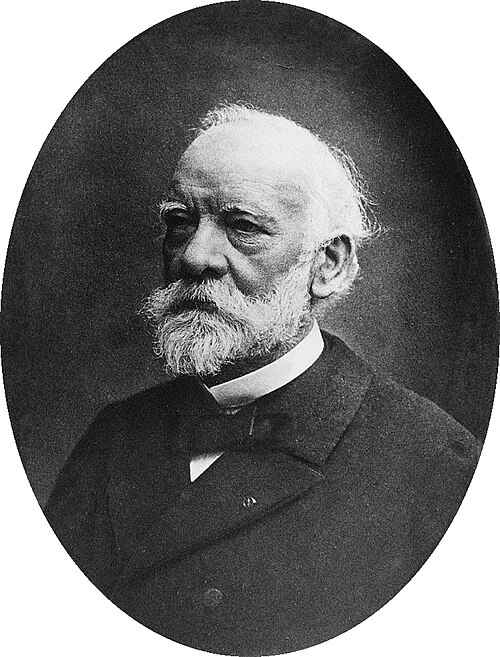
\includegraphics[width=\linewidth]{images/book3/friedel.jpg}
\end{minipage}\hspace{0.02\linewidth}%
\begin{minipage}[t]{0.18\linewidth}
\vspace{0pt}
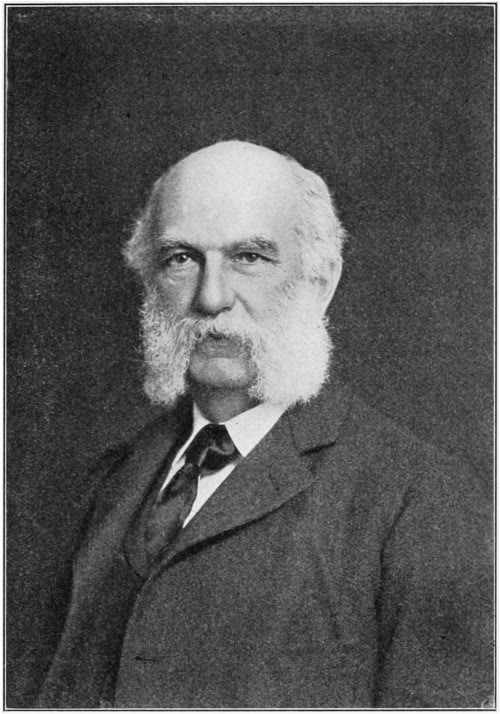
\includegraphics[width=\linewidth]{images/book3/crafts.jpg}
\end{minipage}\hfill
\begin{minipage}[t]{0.58\linewidth}
\vspace{0pt}
In 1877 ontdekten Charles Friedel en James Mason Crafts, die samen in Parijs werkten, dat
aluminiumchloride halogeenalkanen en acylchloriden met benzeen laat reageren. Hun
reacties werden de standaardmanier om koolstofgroepen aan \omterm{def:b2:huckel:aromatic}{aromatische} ringen te hechten, en de
lewiszuurkatalyse die ze ontdekten reikte veel verder. (Portretten: Friedel, jaren 1890; Crafts, uit
\textit{Popular Science Monthly}, 1900; publiek domein, Wikimedia Commons.)
\end{minipage}
\end{history}

\begin{safety}{\ghs[5mm]{GHS02}\,\ghs[5mm]{GHS05}\,\ghs[5mm]{GHS06}\,\ghs[5mm]{GHS08}}
Benzeen is kankerverwekkend en wordt waar mogelijk vervangen door tolueen of andere arenen.
Geconcentreerd salpeterzuur en zwavelzuur zijn corrosief en het nitreermengsel is sterk
oxiderend; het wordt gekoeld en het \omterm{def:b2:aromatic-substitution:arene}{areen} wordt langzaam toegevoegd, want nitreringen zijn \omterm{def:b2:reaction-enthalpy:exothermic}{exotherm}.
Broom is zeer giftig en corrosief; aluminiumchloride reageert heftig met water. Nitroarenen
zijn giftig.
% ledger: ghs:benzene, ghs:toluene, ghs:HNO3, ghs:H2SO4, ghs:Br2, ghs:AlCl3, ghs:nitrotoluene-4
\end{safety}

\section{Oefeningen}

\begin{exercise}[$\star$]\label{exo:b2:aromatic-substitution:1}
Schrijf de vorming van het nitroniumion uit salpeterzuur en zwavelzuur op.
\end{exercise}

\begin{exercise}[$\star$]\label{exo:b2:aromatic-substitution:2}
Geef de hoofdproducten van de bromering (\ce{Br2}, \ce{FeBr3}) van tolueen en van
nitrobenzeen.
\end{exercise}

\begin{exercise}[$\star$]\label{exo:b2:aromatic-substitution:3}
Deel in als activerend of desactiverend, ortho/para of meta: \ce{-CH3}, \ce{-OH}, \ce{-Cl},
\ce{-NO2}, \ce{-COCH3}, \ce{-NHCOCH3}.
\end{exercise}

\begin{exercise}[$\star$]\label{exo:b2:aromatic-substitution:4}
Geef het product van benzeen met ethanoylchloride en aluminiumchloride.
\end{exercise}

\begin{exercise}[$\star\star$]\label{exo:b2:aromatic-substitution:5}
Benzeen en 1-chloorpropaan geven met \ce{AlCl3} vooral isopropylbenzeen. Leg uit, en geef een
route in twee stappen naar propylbenzeen.
\end{exercise}

\begin{exercise}[$\star\star$]\label{exo:b2:aromatic-substitution:6}
Fenol ontkleurt broomwater onmiddellijk, zonder katalysator, en geeft
2,4,6-tribroomfenol. Leg uit.
\end{exercise}

\begin{exercise}[$\star\star$]\label{exo:b2:aromatic-substitution:7}
Geef syntheses van 3-broomnitrobenzeen en 4-broomnitrobenzeen uit benzeen.
\end{exercise}

\begin{exercise}[$\star\star$]\label{exo:b2:aromatic-substitution:8}
Aniline laat zich slecht nitreren (oxidatie, en metaproduct), maar aceetanilide geeft vooral
4-nitroaceetanilide. Verklaar beide feiten.
\end{exercise}

\begin{exercise}[$\star\star$]\label{exo:b2:aromatic-substitution:9}
Toon hoe een sulfonzuurgroep gebruikt kan worden om 2-broomtolueen zonder zijn para-isomeer te bereiden.
\end{exercise}

\begin{exercise}[$\star\star\star$]\label{exo:b2:aromatic-substitution:10}
Waar ondergaat 4-methylanisool (4-methoxytolueen) nitrering? Verklaar met de twee
sturende groepen.
\end{exercise}

\begin{exercise}[$\star\star\star$]\label{exo:b2:aromatic-substitution:11}
2,4,6-Trinitrotolueen wordt gemaakt door drie opeenvolgende nitreringen van tolueen, elk onder strengere
omstandigheden. Leg uit waarom.
\end{exercise}

\begin{exercise}[$\star\star\star$]\label{exo:b2:aromatic-substitution:12}
Stel een synthese voor van 4-nitrobenzoëzuur uit tolueen, en van 3-nitrobenzoëzuur.
\end{exercise}

\section{Probleem: tolueen nitreren}

\begin{problem}[{Weekendprobleem --- het nitroniumion en het mechanisme van de nitrering, de
ortho-, meta- en paraposities van tolueen tegenover de statistische verhouding, de scheiding van de
isomeren, en een massabalans}]
\label{pb:b2:aromatic-substitution:1}
Gegevens: smeltpunten: 2-nitrotolueen \qty{-10}{\degreeCelsius}, 3-nitrotolueen
\qty{16}{\degreeCelsius}, 4-nitrotolueen \qty{52}{\degreeCelsius}. Gegevens voor de oefening, voor één run:
\qty{100}{g} tolueen, \omterm{def:b2:continuous-reactors:conversion}{conversie} 90~\%, isomeerverdeling 58~\% ortho, 4~\% meta,
38~\% para. Molaire massa's (\unit{g/mol}): C 12.011, H 1.008, N 14.007, O 15.999.
% ledger: mp:2-nitrotoluene, mp:3-nitrotoluene, mp:4-nitrotoluene, aw:C, aw:H, aw:N, aw:O

\medskip
\noindent\textbf{Deel I --- Het elektrofiel en het mechanisme.}
\begin{enumerate}
  \item Schrijf de vorming van het nitroniumion op.
  \item Teken zijn lewisstructuur en geef zijn vorm.
  \item Schrijf de aanval van \ce{NO2+} op tolueen para ten opzichte van de methylgroep op.
  \item Teken de drie resonantiestructuren van het \omterm{def:b2:aromatic-substitution:seAr}{para-whelandintermediair}.
  \item Welke stap is snelheidsbepalend?
  \item Wat haalt het proton weg in de tweede stap?
\end{enumerate}

\medskip
\noindent\textbf{Deel II --- De drie posities.}
\begin{enumerate}[resume]
  \item Hoeveel ortho-, meta- en paraposities heeft tolueen?
  \item Welke verhouding zou een willekeurige aanval geven?
  \item Teken het \omterm{def:b2:aromatic-substitution:seAr}{meta-whelandintermediair} en leg uit waarom het het minst gestabiliseerd is.
  \item Hoe stabiliseert de methylgroep het ortho- en het para-intermediair?
  \item Vergelijk de waargenomen verhouding met de statistische: welke posities worden begunstigd?
  \item Vergelijk de opbrengst per positie op ortho (de helft van het orthopercentage) en op para.
        Geef een mogelijke reden voor het verschil.
  \item Wordt tolueen sneller of trager genitreerd dan benzeen?
\end{enumerate}

\medskip
\noindent\textbf{Deel III --- Scheiding.}
\begin{enumerate}[resume]
  \item Welk isomeer is vast bij kamertemperatuur?
  \item Geef aan hoe je het door afkoelen uit het mengsel kunt isoleren.
  \item Waarom begunstigt symmetrie een hoog smeltpunt?
  \item Hoe kunnen het ortho- en het meta-isomeer daarna gescheiden worden?
  \item Waarom zijn deze isomeren moeilijk te scheiden door eenvoudige destillatie?
\end{enumerate}

\medskip
\noindent\textbf{Deel IV --- Massabalans.}
\begin{enumerate}[resume]
  \item Bereken de molaire massa van tolueen en van nitrotolueen.
  \item Bereken de hoeveelheid tolueen en de hoeveelheid gevormd nitrotolueen.
  \item Bereken de massa's van de drie isomeren.
  \item Welke verdere reactie moet vermeden worden door te koelen en geen overmaat zuur te gebruiken?
  \item Hoe zou je 4-nitrobenzoëzuur maken uit het para-isomeer?
  \item Geef de massa 4-nitrotolueen die in deze run uit \qty{100}{g} tolueen verkregen wordt.
\end{enumerate}
\end{problem}
